% !TEX root = main.tex
\section{Dawna implementacja modułu AthenaMonitoring}
Dotychczas środowisko Athena używało jednowątkowego przetwarzania algorytmów.~\cite{tbold-hab-thesis}~\cite{atlas-multithread-presentation}
Ich sekwencja wykonania jest z góry określona przez pliki konfiguracyjne napisane w Athena Python. 
Służą one również do wystartowania całego zadania, np. rekonstrukcji. 
Algorytmy współdzielą dane poprzez pisanie i odczytywanie ich ze wspólnego magazynu danych (Event Store). 
Mogą one również używać narzędzi, które są konfigurowane niezależnie. 
Algorytmy mogą wchodzić w interakcję z serwisami, których cykl życia jest niezależny od cyklu wykonania algorytmów.
W kontekście tej pracy i monitorowania zmiennych, najważniejszy jest serwis do obsługi histogramów - THistSvc.
Zajmuje się tworzeniem i zarządzaniem cyklem życia obiektów z frameworka ROOT.
Schemat wykonania rekonstrukcji został pokazany na rysunku~\ref{fig:athena:oldFlow}.

\begin{figure}[!ht]
\centering
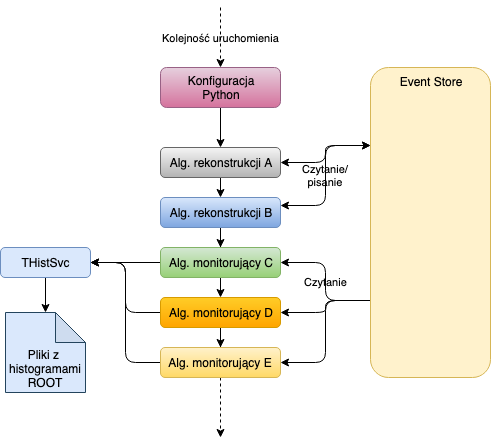
\includegraphics[width=0.75\textwidth]{img/old_flow.png}
\caption{
Schemat prezentuje proces wykonania kodu w aktualnej implementacji środowiska Athena. 
Kolejność algorytmów jest sztywno zdefiniowana w pliku konfiguracyjnym, w którym algorytmy monitorujące wykonywane są po algorytmach rekonstrukcji, które te dane produkują. 
Następnie algorytmy monitorujące komunikują się z serwisem THistSvc w celu zapisania gotowych histogramów do plików ROOT.
}
\label{fig:athena:oldFlow}
\end{figure}

Taka implementacja modułu do monitorowania i algorytmów niesie za sobą następujące niepożądane konsekwencje:

\begin{itemize}
\item twórca algorytmu ma bezpośredni i nieograniczony dostęp do wskaźników na histogramy ROOT. 
W związku z tym, niemożliwe jest zarządzanie takim kodem z centralnego miejsca.
Jego użytkownik, w każdej chwili, może wpłynąć na jego zachowanie i zmienić parametry wykonania.
Co więcej, adaptacja do nowych wersji ROOTa jest całkowicie zależna od autora algorytmu. 
Powoduje to, że framework musi zawsze zachowywać kompatybilność wsteczną, żeby kod Athena nie przestał działać.
Z tego powodu klasy ROOT rozrastają się do kilku tysięcy linii.
\item deklaracja parametrów histogramów dzieje się w kodzie C++ napisanym przez użytkownika. 
W związku z tym drobne zmiany i poprawki binowania histogramów, wymagają nowej wersji frameworka Athena. 
Jest to szczególnie uciążliwe, gdy warunki uruchomienia dynamicznie się zmieniają, a nieprawidłowe binowanie prowadzi np. do umieszczenia w większości wyników poza zakresem.
\item najczęściej używanymi klasami z frameworka ROOT są TH1, TGraph, TTree. 
Ich interfejs jest do siebie bardzo zbliżony. 
Jednakże każdy z tych typów wymaga specjalnego kodu do ich poprawnej obsługi. 
Więc jeśli programista nie będzie postępował dokładnie z wytycznymi z dokumentacji, może to prowadzić do trudnych do wykrycia błędów. 
\end{itemize}

\subsection{Problem scalania histogramów}
Największym problemem aktualnego rozwiązania jest brak możliwości bezpiecznego zapisu z wielu wątków do histogramów ROOT.
Spowodowane jest to implementacją tego frameworka, które nie przewiduje takiego przypadku użycia. 

Kod algorytmów w większości przypadków mógłby zostać łatwo zrównoleglony.
Jednak to, że produkowane przez nie dane muszą zostać umieszczone na histogramie, znacznie utrudnia to zadanie.
Potrzeby jest zewnętrzny mechanizm synchronizacji tych danych, w celu zachowania ich spójności przy umieszczaniu na histogramie.
Obecnie nie ma żadnego ogólnie przyjętego sposobu, który by to umożliwiał.
O ile w ramach jednego algorytmu, byłoby możliwe napisanie niestandardowej synchronizacji, to nie zapewniałaby ona spójności pomiędzy różnymi algorytmami.

Możliwym rozwiązaniem tego problemu mogłyby być histogramy cząstkowe.
Każda instancja algorytmu produkowałaby histogram tylko dla swojej części danych.
Umożliwiłoby to wielowątkową pracę algorytmów, jednak takie rozwiązanie przenosi problem w inne miejsce. 
Konieczne byłoby stworzenie zewnętrznego programu, który scalałby wyniki do ich ostatecznej formy.
Takie narzędzie byłoby mało elastyczne i czasochłonne w stworzeniu i utrzymaniu; konieczność aktualizacji dla różnych przypadków użycia i dodatkowa warstwa w której mogą wystąpić błędy. 
Dodatkowo nie pozwalałoby ono na zaawansowane przypadki użycia histogramów ze względu na separację danych.